%%%%%%%%%%%%%%%%%%%%%%%%%%%%%%%%%%%%%%%%%%%%%%%%%%%%%%%%%%%%%%%%%%%%%%%%%%%%%%%%%%%%
% Document data
%%%%%%%%%%%%%%%%%%%%%%%%%%%%%%%%%%%%%%%%%%%%%%%%%%%%%%%%%%%%%%%%%%%%%%%%%%%%%%%%%%%%
\documentclass[12pt]{report} %report allows for chapters
\renewcommand\thesection{\arabic{section}} % ignore the title number for sections
%%%%%%%%%%%%%%%%%%%%%%%%%%%%%%%%%%%%%%%%%%%%%%%%%%%%%%%%%%%%%%%%%%%%%%%%%%%%%%%%%%%%




%%%%%%%%%%%%%%%%%%%%%%%%%%%%%%%%%%%%%%%%%%%%%%%%%%%%%%%%%%%%%%%%%%%%%%%%%%%%%%%%%%%%
% Packages
%%%%%%%%%%%%%%%%%%%%%%%%%%%%%%%%%%%%%%%%%%%%%%%%%%%%%%%%%%%%%%%%%%%%%%%%%%%%%%%%%%%%
\usepackage{color, soul, xcolor} % Colored text and highlighting, respectively

%Tikz
\usepackage{tikz-cd} % For commutative diagrams
\usepackage{tikz-3dplot}
\RequirePackage{pgfplots}
\usetikzlibrary{shadows}
\usetikzlibrary{shapes}
\usetikzlibrary{decorations}
\usetikzlibrary{arrows,decorations.markings} 
\usetikzlibrary{quotes,angles}

\usepackage{mathtools}
\usepackage{answers}
\usepackage{setspace}
\usepackage{graphicx}
\usepackage{enumerate}
\usepackage{multicol}
\usepackage{mathrsfs}
\usepackage[margin=1in]{geometry} 
\usepackage{amsmath,amsthm,amssymb}
\usepackage{marvosym,wasysym} %fucking smileys
%%%%%%%%%%%%%%%%%%%%%%%%%%%%%%%%%%%%%%%%%%%%%%%%%%%%%%%%%%%%%%%%%%%%%%%%%%%%%%%%%%%%




%%%%%%%%%%%%%%%%%%%%%%%%%%%%%%%%%%%%%%%%%%%%%%%%%%%%%%%%%%%%%%%%%%%%%%%%%%%%%%%%%%%%
% Shortcuts
%%%%%%%%%%%%%%%%%%%%%%%%%%%%%%%%%%%%%%%%%%%%%%%%%%%%%%%%%%%%%%%%%%%%%%%%%%%%%%%%%%%%
% Number systems
\newcommand{\N}{\mathbb{N}}
\newcommand{\Z}{\mathbb{Z}}
\newcommand{\C}{\mathbb{C}}
\newcommand{\R}{\mathbb{R}}
\newcommand{\Q}{\mathbb{Q}}

% Operators/functions
\newcommand{\id}{\mathrm{Id}}
\DeclareMathOperator{\sech}{sech}
\DeclareMathOperator{\csch}{csch}
%%%%%%%%%%%%%%%%%%%%%%%%%%%%%%%%%%%%%%%%%%%%%%%%%%%%%%%%%%%%%%%%%%%%%%%%%%%%%%%%%%%%




%%%%%%%%%%%%%%%%%%%%%%%%%%%%%%%%%%%%%%%%%%%%%%%%%%%%%%%%%%%%%%%%%%%%%%%%%%%%%%%%%%%%
% Environments
%%%%%%%%%%%%%%%%%%%%%%%%%%%%%%%%%%%%%%%%%%%%%%%%%%%%%%%%%%%%%%%%%%%%%%%%%%%%%%%%%%%%
% Italic font
\newtheorem{theorem}{Theorem}[section]
\newtheorem{lemma}{Lemma}[section]
\newtheorem{corollary}{Corollary}[section]
\newtheorem{axiom}{Axiom}

% Plain font
\theoremstyle{definition}
\newtheorem{definition}{Definition}[section]
\newtheorem{example}{Example}[section]
\newtheorem{remark}{Remark}[section]
\newtheorem{solution}{Solution}
\newtheorem{problem}{Problem}[section]
\newtheorem{question}{Question}[section]
\newtheorem{answer}{Answer}[section]
\newtheorem{exercise}{Exercise}[section]
%%%%%%%%%%%%%%%%%%%%%%%%%%%%%%%%%%%%%%%%%%%%%%%%%%%%%%%%%%%%%%%%%%%%%%%%%%%%%%%%%%%%

\begin{document}

\begin{center}
   \textsc{\large MATH 255, Homework 1: \emph{Solutions}}\\
   Due February 1st
\end{center}
\vspace{.5cm}

\noindent\textbf{New Reading:} Read sections 16.5, 16.6, 17.1, 17.2, 17.3

\noindent\textbf{Relevant Sections:} 16.1, 16.2, 16.3, 16.5, 16.6, 16.10.\\

\noindent\textbf{Problem 1.} The \emph{triangle inequality} states that for vectors $\textbf{a}$ and $\textbf{b}$, we have $\|\textbf{a}\|+\|\textbf{b}\|\geq \|\textbf{a}+\textbf{b}\|$. Find an example of a pair $\textbf{a},\textbf{b}$ where strict inequality holds. Find an example of a pair $\textbf{c},\textbf{d}$ where equality holds. Draw a picture for both cases.
\begin{solution}
I will work with vectors in $\R^2$ for simplicity. However, this statement is true in broad generality.

Take the following:
\begin{align*}
    \mathbf{a}&= \begin{bmatrix} 1\\ 1 \end{bmatrix}&
    \mathbf{b}&= \begin{bmatrix} 1\\ 1 \end{bmatrix}\\
    \mathbf{c}&= \begin{bmatrix} 1\\ 0 \end{bmatrix}&
    \mathbf{d}&= \begin{bmatrix} 0\\ 1 \end{bmatrix}.
\end{align*}
Then we can compute both sides of the inequality for the two cases. 
\begin{itemize}
    \item We have
    \begin{align*}
    \|\mathbf{a}\|&=\sqrt{1^2+1^2}=\sqrt{2},\\
    \|\mathbf{b}\|&=\sqrt{1^2+1^2}=\sqrt{2},\\
    \|\mathbf{a}+\mathbf{b}\|&= \sqrt{2^2+2^2}=\sqrt{8}=2\sqrt{2}.
    \end{align*}
        \begin{center}
        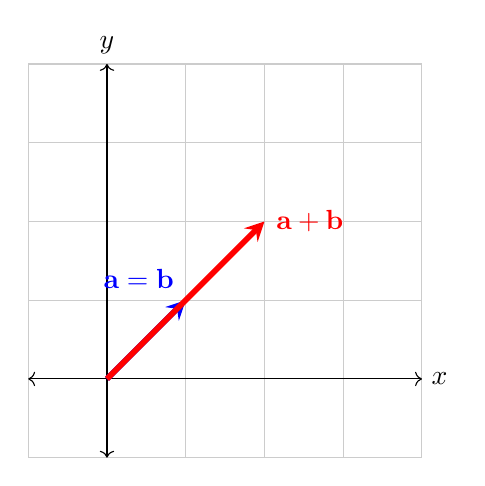
\begin{tikzpicture}
        \draw[thin,gray!40] (-1,-1) grid (4,4);
        \draw[<->] (-1,0)--(4,0) node[right]{$x$};
        \draw[<->] (0,-1)--(0,4) node[above]{$y$};
        \draw[line width=2pt,blue,-stealth](0,0)--(1,1) node[anchor=south east] at (1,1){$\mathbf{a}=\mathbf{b}$};
        \draw[line width=2pt, red, -stealth](0,0)--(2,2) node[anchor=west] at (2,2){$\mathbf{a}+\mathbf{b}$};
        \end{tikzpicture}
        \end{center}
    
    Then we have equality since
    \[
    \underbrace{\|\mathbf{a}\|}_{=\sqrt{2}}+\underbrace{\|\mathbf{b}\|}_{=\sqrt{2}}=\underbrace{\|\mathbf{a}+\mathbf{b}\|}_{=2\sqrt{2}}.
    \]
    In fact, if we consider any two vectors that are pointed in the same direction (including sign, so the angle between them is $0$ and not $\pi$), then this equality holds.
    
    \item We have
    \begin{align*}
    \|\mathbf{c}\|&=\sqrt{1^2+0^2}=1,\\
    \|\mathbf{d}\|&=\sqrt{0^2+1^2}=1,\\
    \|\mathbf{c}+\mathbf{d}\|&= \sqrt{1^2+1^2}=\sqrt{2}.
    \end{align*}
        \begin{center}
        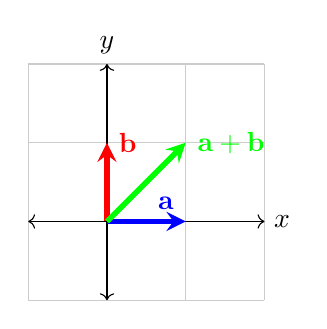
\begin{tikzpicture}
        \draw[thin,gray!40] (-1,-1) grid (2,2);
        \draw[<->] (-1,0)--(2,0) node[right]{$x$};
        \draw[<->] (0,-1)--(0,2) node[above]{$y$};
        \draw[line width=2pt,blue,-stealth](0,0)--(1,0) node[anchor=south east] at (1,0){$\mathbf{a}$};
        \draw[line width=2pt, red, -stealth](0,0)--(0,1) node[anchor=west] at (0,1){$\mathbf{b}$};
        \draw[line width=2pt, green, -stealth](0,0)--(1,1) node[anchor=west] at (1,1){$\mathbf{a}+\mathbf{b}$};
        \end{tikzpicture}
        \end{center}
    
    Then we have the inequality since
    \[
    \underbrace{\|\mathbf{c}\|}_{=1}+\underbrace{\|\mathbf{c}\|}_{=1}>\underbrace{\|\mathbf{c}+\mathbf{d}\|}_{=\sqrt{2}}.
    \]
    There are many other options here. Another good one to consider would be
    \begin{align*}
            \mathbf{c}&= \begin{bmatrix} 1\\ 0 \end{bmatrix}&
    \mathbf{d}&= \begin{bmatrix} -1\\ 0 \end{bmatrix}.
    \end{align*}
    Check what happens here for yourself.
\end{itemize}
\end{solution}
\hspace{.5cm}

\noindent\textbf{Problem 2.} Let $\textbf{a}=(1,3)$, and $\textbf{b}=(5,2)$ be vectors with initial point at the origin and terminal points of $A$ and $B$ respectively. Find a vector that bisects the line segment $AB$ and compute its unit vector.
\begin{solution}
Let us first draw a picture of this situation:
        \begin{center}
        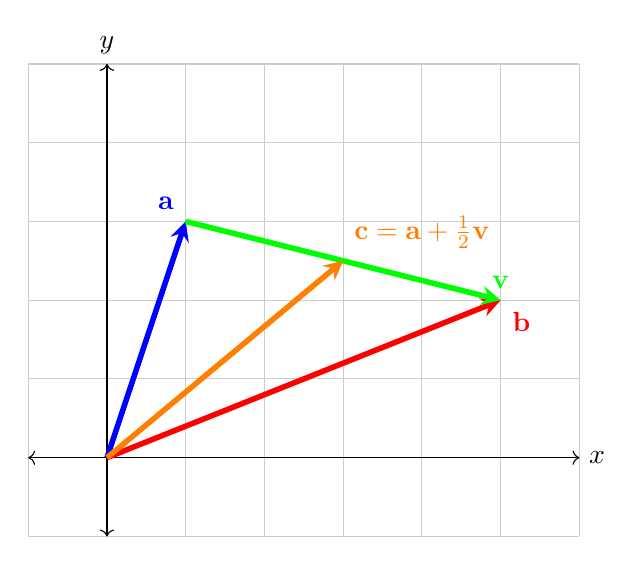
\begin{tikzpicture}
        \draw[thin,gray!40] (-1,-1) grid (6,5);
        \draw[<->] (-1,0)--(6,0) node[right]{$x$};
        \draw[<->] (0,-1)--(0,5) node[above]{$y$};
        \draw[line width=2pt,blue,-stealth](0,0)--(1,3) node[anchor=south east] at (1,3){$\mathbf{a}$};
        \draw[line width=2pt, red, -stealth](0,0)--(5,2) node[anchor=north west] at (5,2){$\mathbf{b}$};
        \draw[line width=2pt, green, -stealth](1,3)--(5,2) node[anchor=south] at (5,2){$\mathbf{v}$};
        \draw[line width=2pt, orange, -stealth](0,0)--(3,2.5) node[anchor=south] at (4,2.5){$\mathbf{c}=\mathbf{a}+\frac{1}{2}\mathbf{v}$};
        \end{tikzpicture}
        \end{center}
        Our goal is to find a unit vector $\mathbf{u}$ in the same direction as $\mathbf{c}$ we have in the illustration above.  
        
        To get to the midpoint of the line segment between the points $\mathbf{a}$ and $\mathbf{b}$ we can walk along $\mathbf{a}$ and halfway along the vector $\mathbf{v}$ drawn above to get to $\mathbf{c}$.  That is to say
        \[
        \mathbf{c}=\mathbf{a}+\frac{1}{2}\mathbf{v}.
        \]
        We find $\mathbf{v}$ by taking the vector difference between $\mathbf{b}$ and $\mathbf{a}$.  So
        \[
        \mathbf{v}=\mathbf{b}-\mathbf{a}=(4,-1).
        \]
        Of course, $\mathbf{v}$ really sits with its tail at the origin $(0,0)$, but we should feel free to move it to the head of $\mathbf{a}$ as in the figure.
        
        We compute the length of $\mathbf{c}$
        \[
        \|\mathbf{c}\|=\sqrt{3^2+2.5^2}=\sqrt{15.25}. 
        \]
        To get the unit vector $\mathbf{u}$ pointing in the direction of $\mathbf{c}$, we then take
        \[
        \mathbf{u}=\frac{1}{\|\mathbf{c}\|}\mathbf{c}=\left( \frac{3}{\sqrt{15.25}},\frac{2.5}{\sqrt{15.25}}\right).
        \]
        
        Another way to interpret this is $\mathbf{c}$ is the average position of the vectors $\mathbf{a}$ and $\mathbf{b}$ as it lies in the midpoint on the line between them.  Using this, we can see
        \[
        \mathbf{c}=\frac{1}{2}\mathbf{a}+\frac{1}{2}\mathbf{b}=\mathbf{a}+\frac{1}{2}\mathbf{v}.
        \]
        Both ways give the same answer, but have a bit of a different approach.  
\end{solution}
\hspace{.5cm}

\noindent\textbf{Problem 3.} Suppose three masses $m_1 = 2$, $m_2 = 3$, $m_3 = 10$ have respective position vectors $\textbf{p}_1 = (1,0,4)$, $\textbf{p}_2 = (0,3,2)$, and $\textbf{p}_3 = (2,2,0)$. What position vector $\textbf{p}_4$ should be assigned to a fourth mass $m_4 = 2$ so that the center of mass of the whole system is at the origin?
\begin{solution}
It's a good idea to think of a picture in your head. All of these masses are positive (or zero) in each component. This should lead you to believe that you must have to put this last mass, $m_4$, in a place where each component is negative.  In the 1D case, if we put all the mass on one side of a see-saw, then we must have to put the last mass on the other side in order for the see-saw to rest at equilibrium.

Algebraically, we will have an equation that tells us the $x$-component for $\mathbf{p}_4$, an equation for the $y$-component, and $z$-component as well.  The center of mass equation for our situation reads:
\[
\underbrace{\mathbf{R}_{cm}=\frac{1}{m_1+m_2+m_3+m_4}(m_1\mathbf{p}_1+m_2\mathbf{p}_2+m_3\mathbf{p}_3+m_4}_{\textrm{known information}}\mathbf{p}_4).
\]
The only unknown here is $\mathbf{p}_4$. We want $\mathbf{R}_{cm}=\mathbf{0}$, and we can plug in the known values to get
\[
\begin{bmatrix} 0\\ 0\\ 0\end{bmatrix}
= \frac{1}{17}\left(2
\begin{bmatrix} 1\\ 0\\ 4\end{bmatrix}+
3\begin{bmatrix} 0\\ 3\\ 2\end{bmatrix}+
10\begin{bmatrix} 2\\ 2\\ 0\end{bmatrix}+
2\begin{bmatrix} x\\ y\\ z\end{bmatrix}\right).
\]
We can multiply both sides by $17$ and compute this linear combination above to find
\[
\begin{bmatrix} 0\\ 0\\ 0 \end{bmatrix}=
\begin{bmatrix} 22+2x\\ 29+2y\\ 14+2z\end{bmatrix}.
\]
This gives us an equation for $x$, $y$, and $z$, all of which we know how to solve. That is
\begin{align*}
    0&= 22+2x\\
    0&= 29+2y\\
    0&= 14+2z.
\end{align*}
Solving each gives $x=-11$, $y=-29/2$, and $z=-7$. So we have that
\[
\mathbf{p}_4 = \begin{bmatrix} -11\\ -29/2\\ -7 \end{bmatrix}.
\]
What if $m_4$ had been much heavier? Say, $m_4=20$? Think about the see-saw example.
\end{solution}
\hspace{.5cm}

\noindent\textbf{Problem 4.} Which two of the following vectors have the smallest difference in angle?
\begin{align*}
\textbf{a} = (1,2,3),\; \textbf{b} = (\pi,\pi,1),\; \textbf{c} = (-1,-\pi,3),\; \textbf{d} = (1,-\pi,3).
\end{align*}
\begin{solution}
With problems like this, we want to realize all the work we have to do and go about it in the most efficient way.  What tools do we need to use and which comparisons do we need to make? 

Our tool will be the dot product (both ways of computing this) and we compare the following list:
\begin{itemize}
    \item $\mathbf{a}$ with $\mathbf{b}$,
    \item $\mathbf{a}$ with $\mathbf{c}$,
    \item $\mathbf{a}$ with $\mathbf{d}$,
    \item $\mathbf{b}$ with $\mathbf{c}$,
    \item $\mathbf{b}$ with $\mathbf{d}$,
    \item $\mathbf{c}$ with $\mathbf{d}$.
\end{itemize}
Our two ways of computing the dot product are given by
\[
\mathbf{u}\cdot \mathbf{v} = u_1v_1+u_2v_2+u_3v_3 = \|u\|\|v\|\cos \theta.
\]
We can solve for $\theta$ here and use this formula later.  We get
\[
\theta = \arccos\left( \frac{u_1v_1+u_2v_2+u_3v_3}{\|u\|\|v\|}\right).
\]
Verify this algebra for yourself.  

We also need the length of each vector in order to do this.  So let's go ahead and get those.
\begin{align*}
    \|a\|&=\sqrt{1^2+2^3+3^2}=\sqrt{14}\\
    \|b\|&=\sqrt{\pi^2+\pi^2+1^2}=\sqrt{2\pi^2+1}\\
    \|c\|&=\sqrt{(-1)^2+(-\pi)^2+3^3}=\sqrt{\pi^2+10}\\
    \|d\|&=\sqrt{1^2+(-\pi)^2+3^2}=\sqrt{\pi^2+10}.
\end{align*}
We then use our formula and compute:

\begin{align*}
    \theta_{ab}&=\arccos\left( \frac{(1\cdot \pi)+(2\cdot \pi)+(3\cdot 1)}{\sqrt{14}\cdot\sqrt{2\pi^2+1}}\right)\approx0.7537\approx 43.18^\circ\\
    \theta_{ac}&=\arccos\left( \frac{(1\cdot (-1))+(2\cdot (-\pi))+(3\cdot 3)}{\sqrt{14}\cdot\sqrt{\pi^2+10}}\right)\approx1.4677\approx 84.09^\circ\\
    \theta_{ad}&=\arccos\left( \frac{(1\cdot 1)+(2\cdot (-\pi))+(3\cdot 3)}{\sqrt{14}\cdot\sqrt{\pi^2+10}}\right)\approx1.3461\approx 77.12^\circ\\
    \theta_{bc}&=\arccos\left( \frac{(\pi\cdot (-1))+(\pi \cdot (-\pi))+(1\cdot 3)}{\sqrt{2\pi^2+1}\cdot\sqrt{\pi^2+10}}\right)\approx2.0865\approx 119.5^\circ\\
    \theta_{bd}&=\arccos\left( \frac{(\pi\cdot 1)+(\pi \cdot (-\pi))+(1\cdot 3)}{\sqrt{2\pi^2+1}\cdot\sqrt{\pi^2+10}}\right)\approx1.7555\approx 100.6^\circ\\
    \theta_{cd}&=\arccos\left( \frac{((-1)\cdot 1)+((-\pi) \cdot (-\pi))+(3\cdot 3)}{\sqrt{\pi^2+10}\cdot\sqrt{\pi^2+10}}\right)\approx0.4525\approx 25.93^\circ.
\end{align*}
It seems the largest was the angle $\theta_{bc}$ between the vectors $\mathbf{b}$ and $\mathbf{c}$.  Yes, this was a bit tedious.  It happens.  I used WolframAlpha to compute all of this and it saved me quite some time.  
\end{solution}
\hspace{.5cm}

\noindent\textbf{Problem 5.} Let $\textbf{a} = (-3,7,2)$ and $\textbf{b} = (-1,-1,-5)$. Compute $\textbf{a}\times\textbf{b}$ and show that it is orthogonal to both $\textbf{a}$ and $\textbf{b}$.
\begin{solution}
From our notes, we know the cross product of vectors follows
\[
\mathbf{a}\times \mathbf{b}=(a_yb_z-a_zb_y,a_zb_x-a_xb_z,a_xb_y-a_yb_x).
\]
Using our specific vectors, we find
\[
\mathbf{a}\times \mathbf{b}=(7\cdot(-5)-2\cdot(-1),2\cdot (-1)-(-3)\cdot(-5),(-3)\cdot(-1)-7\cdot(-1))=(-33,-17,10).
\]
I verified this with WolframAlpha.  

To see if this is orthogonal to both $\mathbf{a}$ and $\mathbf{b}$ we simply use the fact that $\mathbf{v}$ and $\mathbf{u}$ are orthogonal if and only if
\[
\mathbf{v}\cdot \mathbf{u}=0.
\]
So we compute this
\begin{align*}
    (\mathbf{a}\times \mathbf{b})\cdot \mathbf{a}&=(-33)\cdot (-3)+(-17)\cdot 7+10\cdot 2= 0\\
    (\mathbf{a}\times \mathbf{b})\cdot \mathbf{b}&=(-33)\cdot (-1)+(-17)\cdot (-1)+10\cdot (-5)= 0.
\end{align*}
Hence, $\mathbf{a}\times \mathbf{b}$ is orthogonal to both $\mathbf{a}$ and $\mathbf{b}$.
\end{solution}
\hspace{.5cm}






































\end{document}  